\documentclass[main.tex]{subfiles}

\begin{document}

\section{Upgradablity}

Once a compiled smart contract binary is deployed on an EVM-compatible blockchain, it becomes immutable, and any modifications to the binary are not possible. OpenZeppelin \cite{proxy} utilizes a proxy-based approach for updates. The specific method involves deploying a proxy smart contract along with all the implementation smart contracts and setting an admin address. When there is a need to update the implementation contract, the admin can directly modify the proxy, redirecting the proxy to the new implementation contract address.

For the DARC protocol, the proxy upgrade pattern is not applicable because it requires setting an admin in the proxy. The admin in the DARC protocol would have complete control and modification rights, potentially overwriting all existing assets, plugins, and information, resulting in the admin's power surpassing that of all token holders at various levels. In a scenario where there is already an established corporate structure in a company, having a super administrator with the authority to modify all legal aspects, deal with all company shares, and manage assets would be a dangerous proposition.

The program entrance serves as the unified and exclusive entry point for the DARC protocol. When upgrading from an old DARC instance X to a new DARC instance Y, the process is streamlined. This involves configuring the upgrade address for the old DARC instance X and setting up the new DARC instance Y to accept all delegate programs from DARC instance X. With these adjustments, the upgrade is smoothly executed. After the upgrade, users can seamlessly continue executing programs in DARC instance X, and these programs will be delegated and executed within the new DARC instance Y.

In the DARC protocol, there are three operations related to upgrades:

\begin{itemize}
    \item \texttt{upgradeToAddress(targetAddress)}: Upgrades the current DARC instance to the targetAddress. All programs submitted to the current DARC instance will be delegated and executed in the DARC instance at the targetAddress.
    
    \item \texttt{confirmUpgradedFromAddress(sourceAddress)}: Allows the current DARC instance to upgrade from the DARC instance at sourceAddress. When a program is proxied and submitted from sourceAddress, it is permitted to run in the current DARC instance with the operator identity of the program submitter.

    \item \texttt{upgradeToTheLatest()}: If the current DARC instance A has been upgraded to the new DARC instance B, and the new DARC instance B has also been upgraded to the updated DARC instance C, executing this function will directly upgrade the DARC instance to DARC instance C. In other words, programs executed in this DARC instance A will be directly delegated and executed in DARC instance C, bypassing DARC instance B. This operation will be interpreted differently. Assuming a DARC instance A has already undergone an upgrade to DARC instance B, in such a scenario, if a user executes a program in A with only one \texttt{upgradeToTheLatest()} operation, the program will be executed in DARC instance A instead of being delegated to DARC instance B.
\end{itemize}

With the three operations mentioned above, we can discuss two scenarios for upgrading the DARC protocol:

In the first scenario, where the user has already deployed My DARC 1, and My DARC 1 has not been upgraded to any other DARC, the following three steps are necessary:

\begin{enumerate}
    \item Deploy the new version of My DARC 2 to the blockchain and complete all configurations.
    \item Execute \texttt{confirmUpgradedFromAddress(MyDARC1Addr)} in My DARC 2, allowing My DARC 2 to accept programs and act as a proxy for My DARC 1.
    \item Execute \texttt{upgradeToAddress(MyDARC2Addr)} in My DARC 1, completing the upgrade from My DARC 1 to My DARC 2.
\end{enumerate}

Figure \ref{fig:upgrade} illustrates the entire process of upgrading directly from My DARC 1 to My DARC 2.


\begin{figure}
\centering
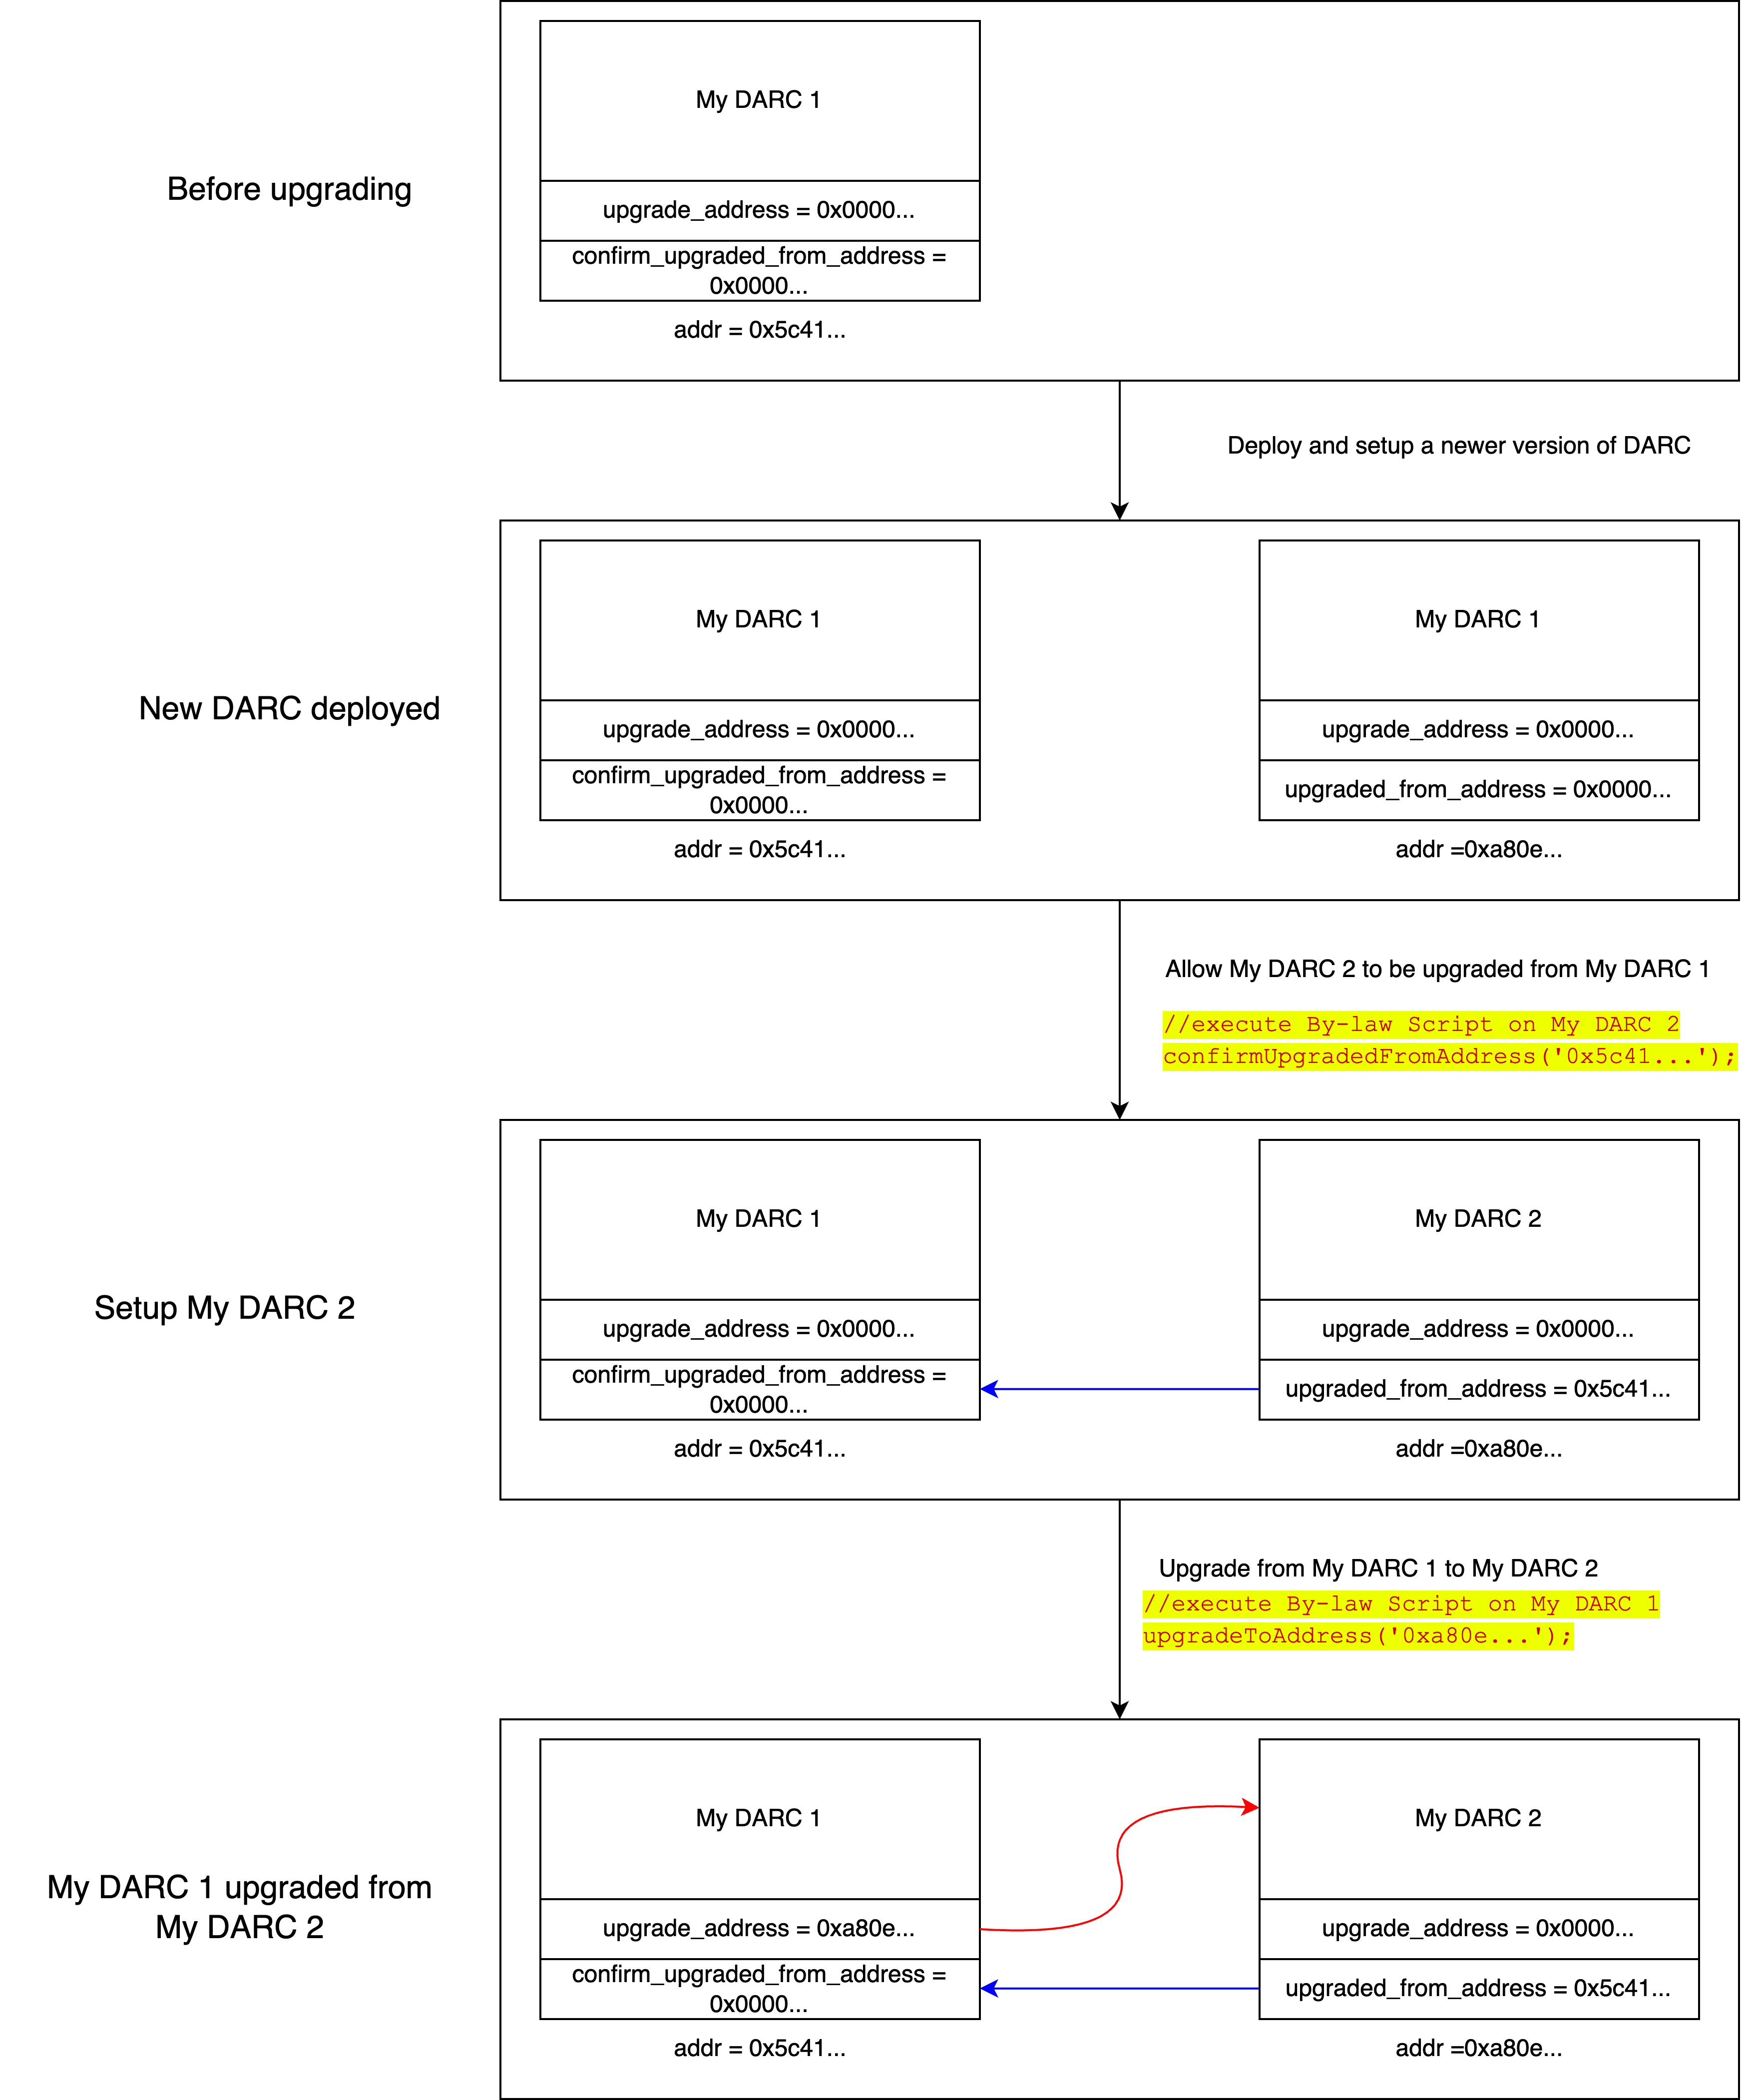
\includegraphics[width=1\linewidth]{upgradability.drawio.png}
\caption{\label{fig:upgrade}Upgrading from My DARC 1 to My DARC 2}
\end{figure}


In the second scenario, where the user has deployed My DARC 1, My DARC 1 has already been upgraded to My DARC 2, and the user intends to further upgrade to My DARC 3, the following three steps are required:

\begin{enumerate}
    \item Deploy the new version of My DARC 3 on the blockchain and complete all configurations.
    \item Execute \texttt{confirmUpgradedFromAddress(MyDARC1Addr)} in My DARC 3, enabling My DARC 3 to accept programs and proxies from My DARC 1.
    \item Execute \texttt{upgradeToAddress(MyDARC2Addr)} in My DARC 1. Since this program will run in My DARC 2 under the proxy of My DARC 1, the \texttt{upgrade\_address} of My DARC 2 will point to the address of My DARC 3.
    \item Execute \texttt{upgradeToTheLatest()} in My DARC 1, directing My DARC 1 to the address of My DARC 3 based on the address of My DARC 2, completing the upgrade from My DARC 1 to My DARC 3.
    \item Finally, close My DARC 2.
\end{enumerate}

Figure \ref{fig:upgrade-multi} illustrates the entire process of upgrading directly from My DARC 1 to My DARC 3.






\begin{figure}
\centering
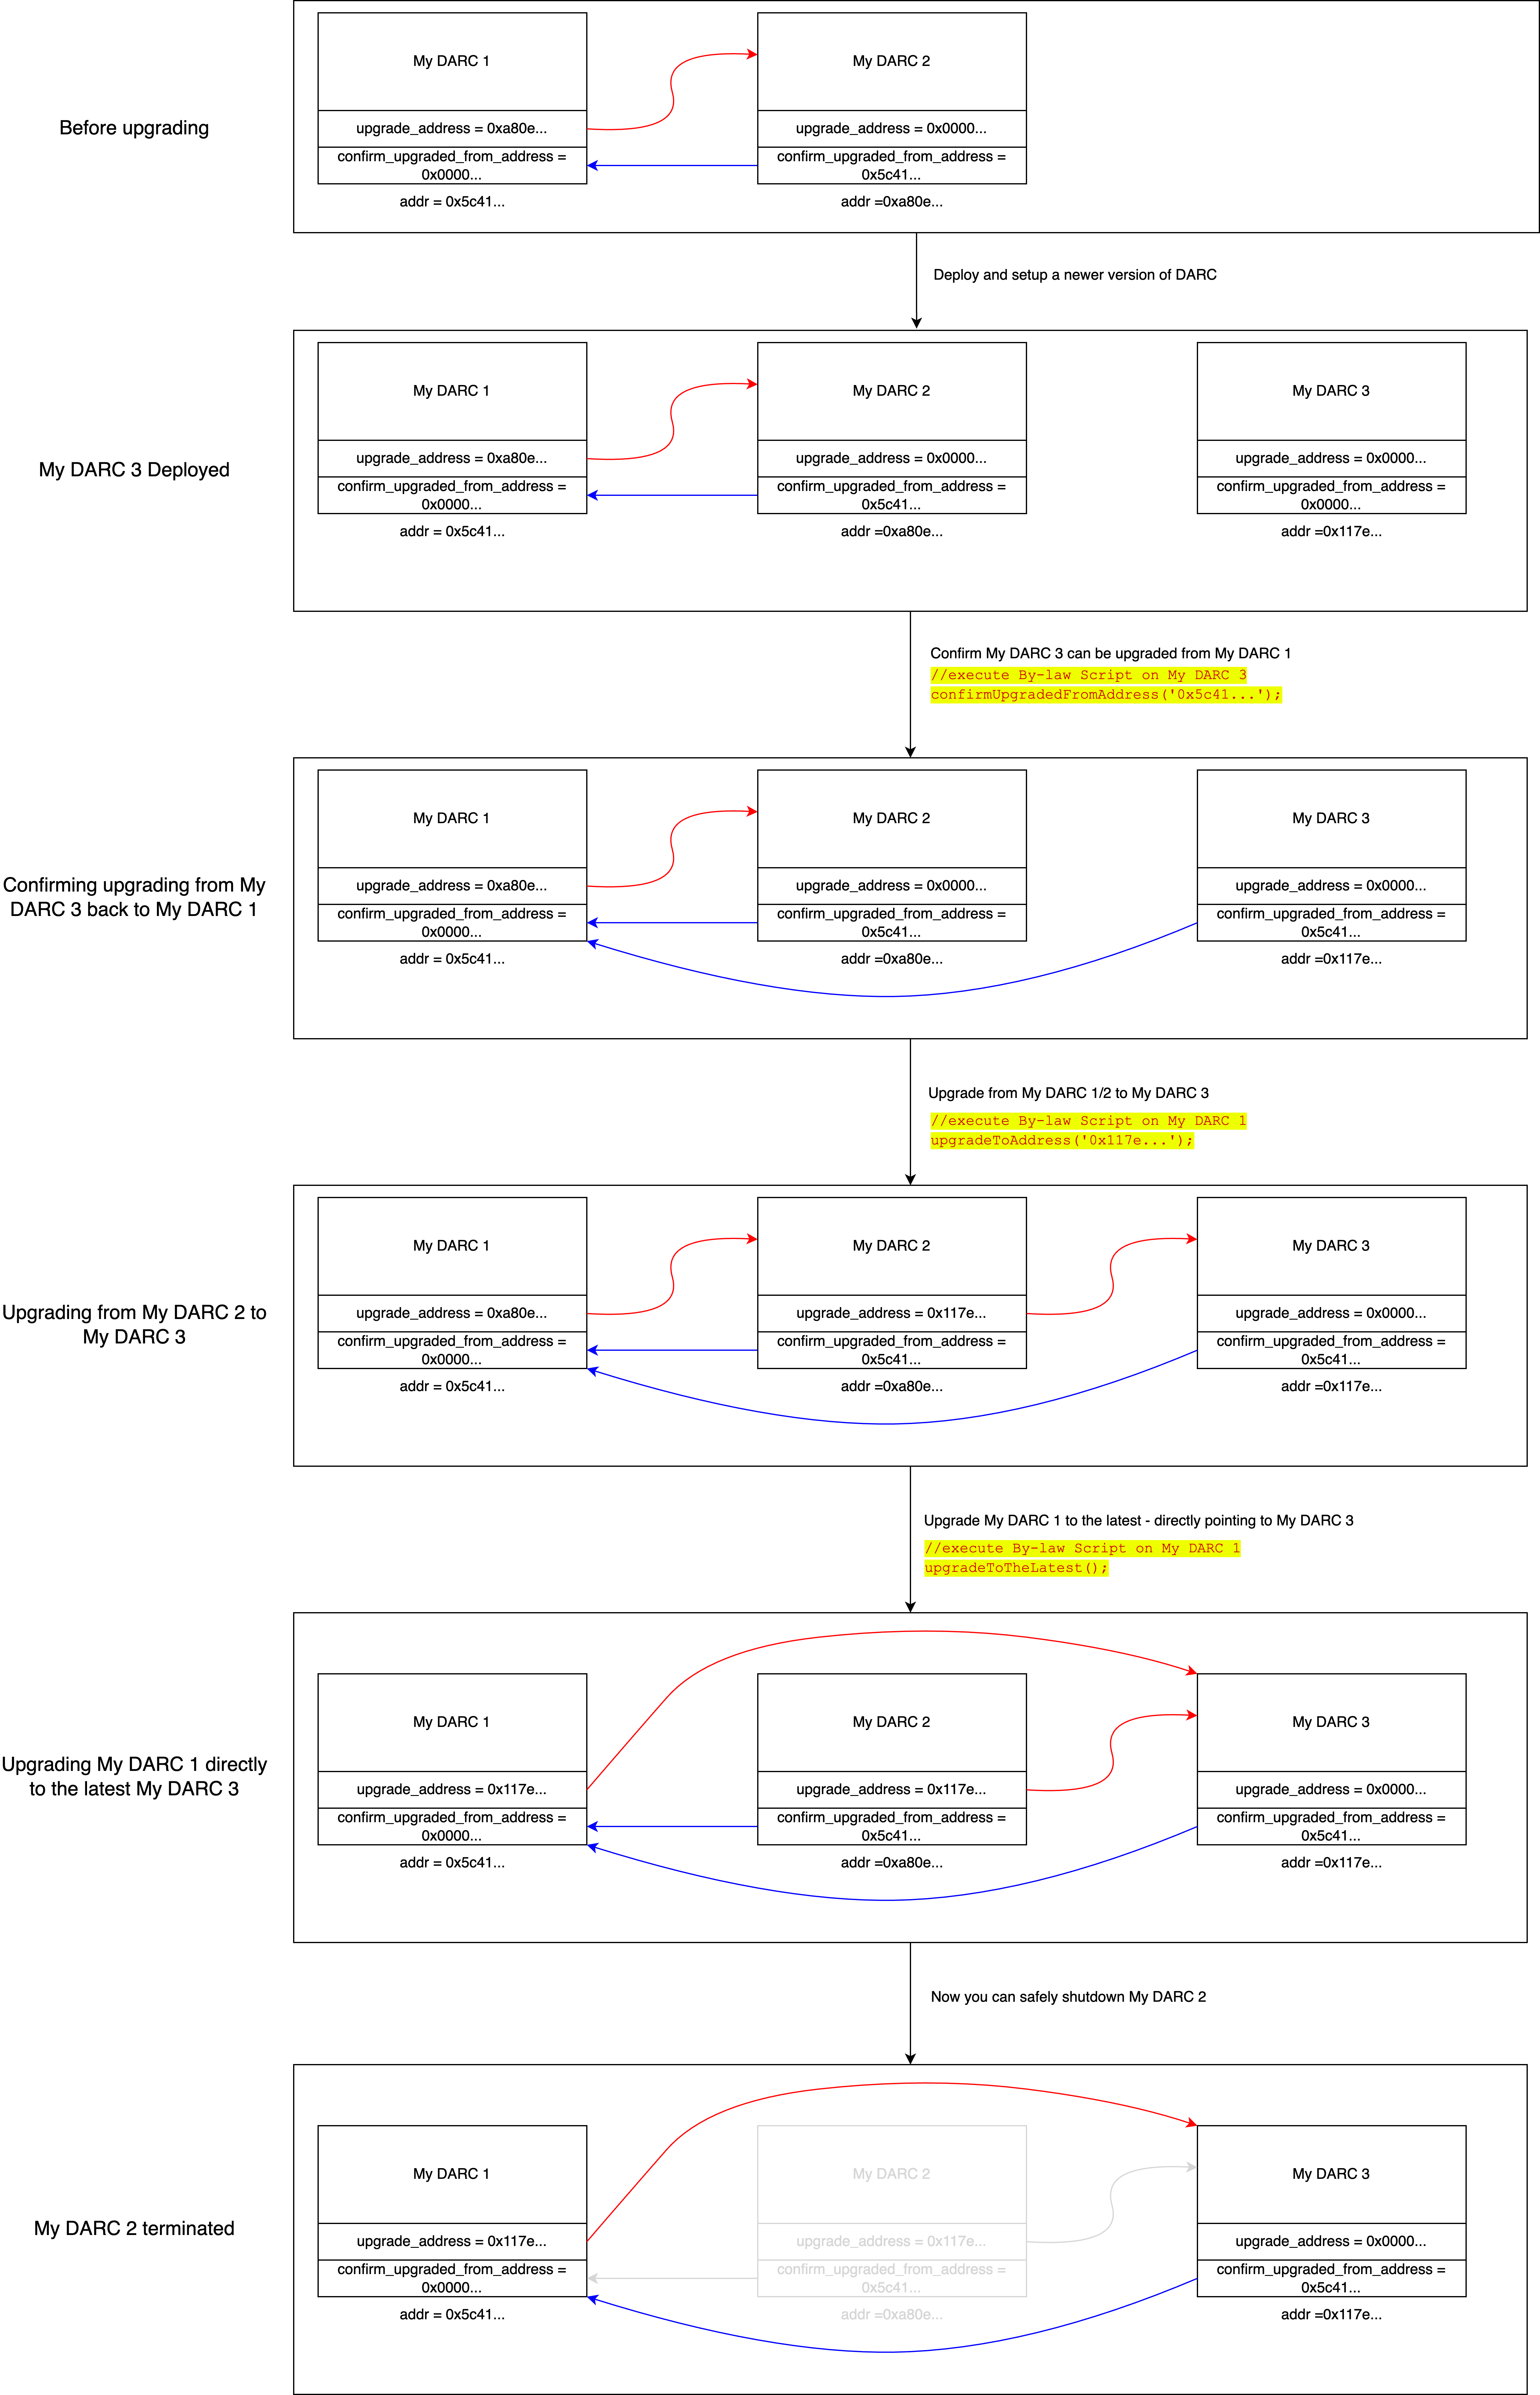
\includegraphics[width=1\linewidth]{upgradablity-multi.drawio.png}
\caption{\label{fig:upgrade-multi}Upgrading from My DARC 1 to My DARC 2 to My DARC 3}
\end{figure}

\end{document}